% My previous "advanced" work
Multi-wave history matching refines the emulator iteratively. Observed data was generated using LHD for an additional wave, incorporating observation errors and model discrepancy. The first step was calculating implausibility metrics across the input space.

Figure~\ref{fig:implausibility} is an implausibility map. High implausibility regions (lighter shade) were excluded from subsequent waves, while low areas (darker shade) guided further sampling.

\begin{figure}[H]
    \centering
    \includegraphics[width=0.6\textwidth]{Implausibility.png}
    \caption{Implausibility map $I(x)$ indicating regions of high and low emulator accuracy.}
    \label{fig:implausibility}
\end{figure}

\noindent Here are a few insights this plot provides:
\begin{itemize}
    \item High implausibility values (lighter regions) appear around \( x_1 \approx 0.2, x_2 \approx 0.2 \) and \( x_1 \approx 0.7, x_2 \approx 0.8 \), indicating areas where the emulator has higher uncertainty.
    \item The majority of the space is dark, suggesting that the emulator performs well across most of the domain.
\end{itemize}

\noindent The presence of high implausibility regions suggests if fewer design points were placed in these areas, the emulator might lack sufficient data for accurate predictions. It also implies the true function may exhibit complex behaviour in these regions, making them more difficult to emulate.

Following the first wave, new design points were added from non-implausible regions, and the emulator was retrained. Figure~\ref{fig:2DMVHM} illustrates the updated expectation surface after the second wave, with lighter regions indicating areas of higher predicted output. This multi-wave approach narrows the parameter space, ensuring that the emulator aligns more closely with observed data.

\begin{figure}[H]
    \centering
    \includegraphics[width=0.6\textwidth]{2DMVHM.png}
    \caption{Multi-Wave History Matching - Emulator response after the second wave.}
    \label{fig:2DMVHM}
\end{figure}
\noindent Here are a few key insights from the plot:
\begin{itemize}
    \item Some areas (e.g., near \(x_1 \approx 0.7, x_2 \approx 0.9\)) still show significant variation, suggesting that more training might be necessary.
    \item It is clear to see how the implausibility map has trained this wave. For example, the top right is primarily a lighter shade in the implausibility, which has been considered in Wave 2 of the multi-wave history matching.
\end{itemize}

\noindent Ultimately, this plot improved upon the initial Emulator expectation, which makes sense because it has already learnt some key features of the data points. In spite of this, there is still room for improvement, so maybe another wave could be applied. See \ref{fig:Wave 2 Emulator Overlay} for the multi-wave history match and initial contour plot overlap.

% Previous Plot Descriptions
\begin{figure}[H]
    \centering
    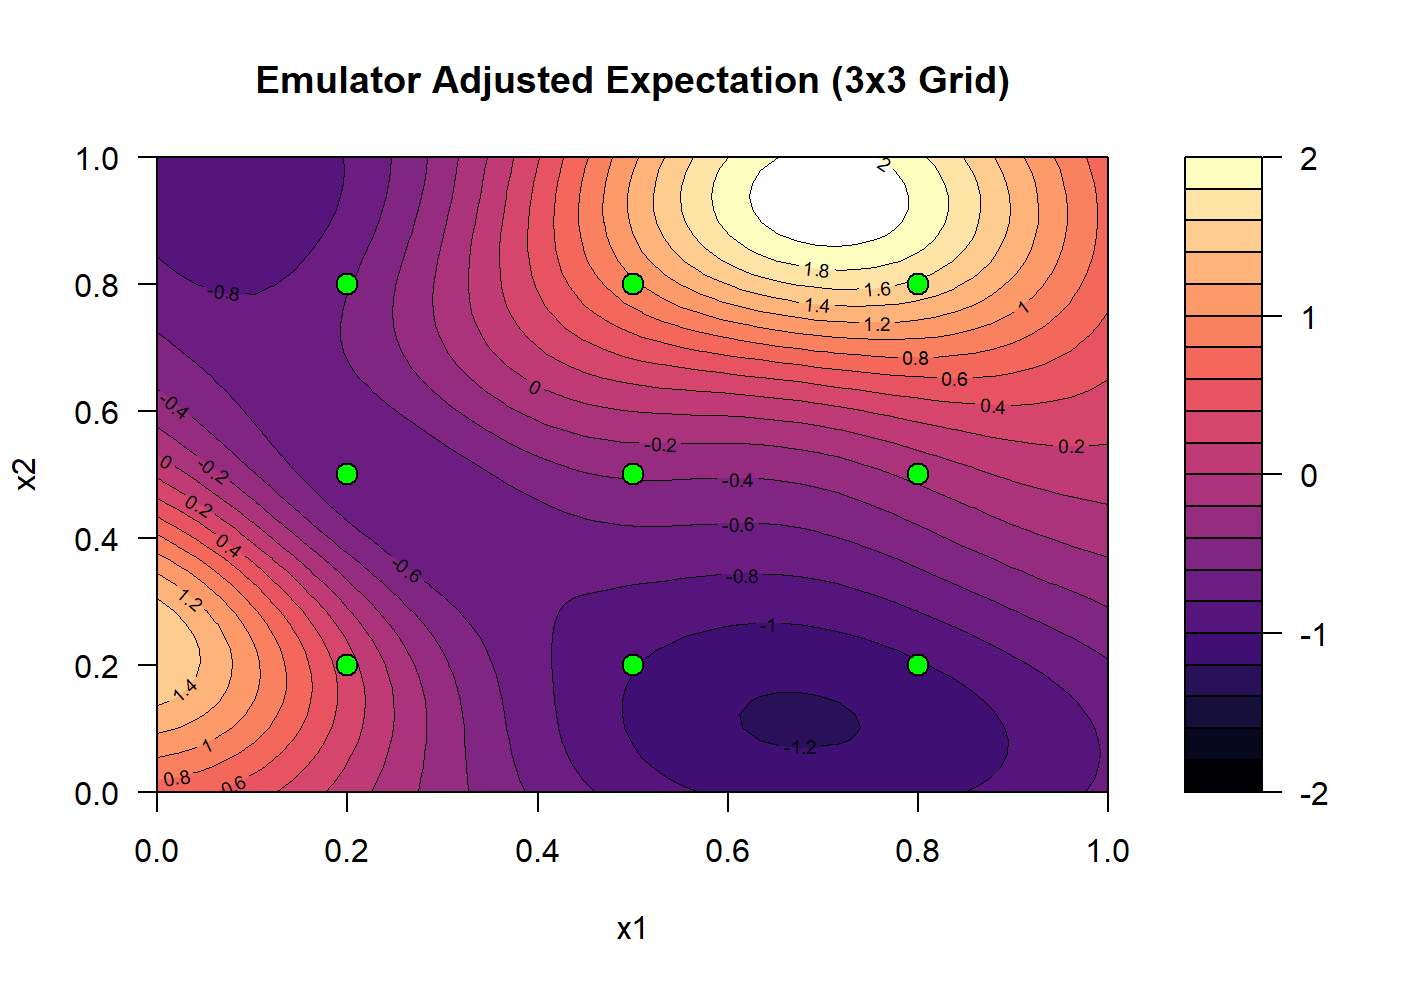
\includegraphics[width=0.8\textwidth]{2D Emulator Expectation.png}
    \caption{2D Emulator Expectation for the response surface across the input space.}
    \label{fig:2d_emulator}
\end{figure}

\noindent The key insights from Figure \ref{fig:2d_emulator} are:

\begin{itemize}
    \item The true function and emulator expectation share the same general trend, with high values in the bottom left and top right and low values (blue regions) lower the upper region. 
    This suggests that the emulator is correctly approximating the large-scale behaviour of the Branin-Hoo function.

    \item The true function has a smoother transition between contour levels, while the emulator output introduces some artificial contour warping. 
    This could be due to limited training points, interpolation smoothness, or kernel settings in the emulator.

    \item The emulator expectation closely follows the true function in high-value regions, such as at \(x_1 \approx 0\), \(x_2 \approx 0\). 
    This suggests that the emulator is well-calibrated in these areas.

    \item The emulator appears to exaggerate some low-value regions compared to the true function. 
    This could indicate that the emulator is slightly overestimating the negative values of the function in certain regions.

    \item If possible, adding more training points in regions where contours change rapidly (e.g., around \(x_1 \approx 0.2, x_2 \approx 0.2\)) might help. 
    Since adjusting hyperparameters is not an option, checking variance plots could help identify areas where the emulator is uncertain.
\end{itemize}

\noindent See \ref{fig:overlay_exp} for the emulator expectation and contour plot overlay for more detail.

Figure \ref{fig:Var} shows a 2D contour map of the variance surface. This plot reveals regions of higher variance (lighter blue) concentrated in specific areas of the input space, indicating lower confidence in the emulator's predictions in those regions. In contrast, darker blue areas correspond to lower variance, suggesting greater confidence in the emulator predictions in those regions.

\begin{figure}[H]
    \centering
    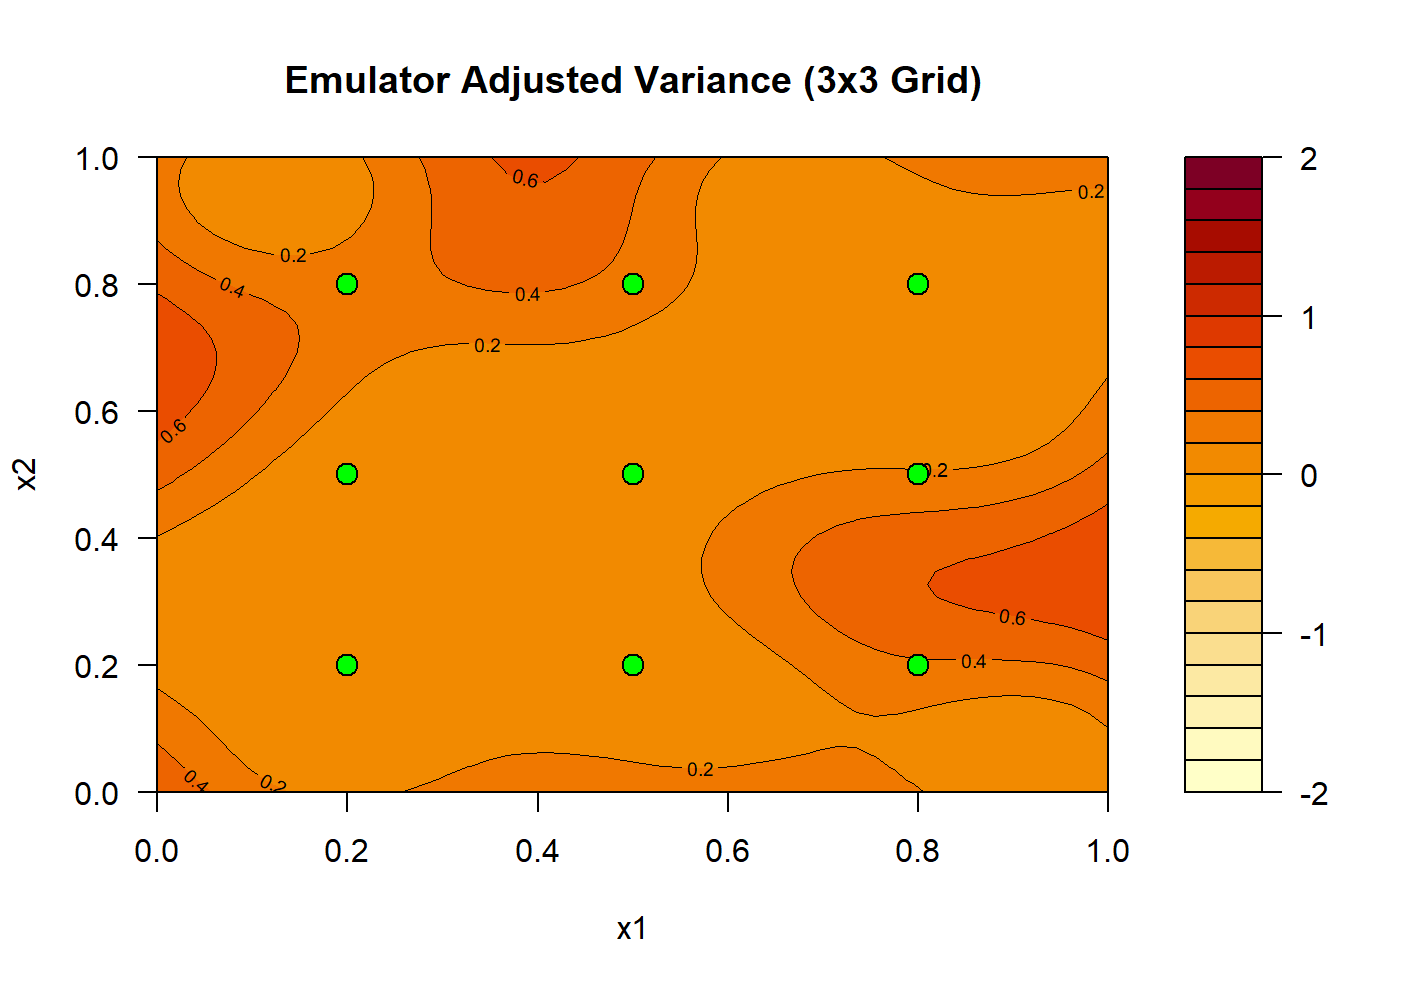
\includegraphics[width=0.7\textwidth]{2D Emulator Variance.png}
    \caption{2D Emulator Variance for the response surface across the input space.}
    \label{fig:Var}
\end{figure}

\noindent The key insights from Figure \ref{fig:Var} are:
\begin{itemize}
    \item Minimal variance (\(< 0.1\)) in areas where the emulator aligns well with the true function, such as \(x_1 \approx 0.2, x_2 \approx 0.2\) and \(x_1 \approx 0.8, x_2 \approx 0.8\), reflecting high confidence in predictions.
    \item Variance increases (\(> 0.4\)) in regions with fewer training points or steep gradients, such as around \(x_1 \approx 0.8, x_2 \approx 0.3\) and \(x_1 \approx 0.4, x_2 \approx 0.9\), indicating emulator prediction uncertainty.
    \item Variance transitions smoothly across the input space, and it is predominantly on the lower end, as shown by the larger representation of darker colours, suggesting the emulator generalises well.
\end{itemize}

%LHS benefits and disadvantages:
Latin Hypercube Sampling (LHS) is stages 1 and 2 of LHD. LHS is used because it improves convergence, which comes from its ability to reduce variance in model outputs. LHS prevents oversampling in localised regions, providing better estimates of the function's mean and variance with fewer samples.\cite{owen1998latin} The variance of the LHS estimator, \( \hat{\mu}_{\text{LHS}} \), converges faster than that of simple random sampling (SRS) \( \hat{\mu}_{\text{SRS}} \): $\text{Var}(\hat{\mu}_{\text{LHS}}) \leq \text{Var}(\hat{\mu}_{\text{SRS}})$ by stratifying each dimension of the input space and creating negative covariance between sample cells, ensuring more uniform coverage.\cite{SHIELDS201696} This is more computationally efficient, and hence, fewer samples are required to achieve the same level of accuracy compared to SRS, making LHS especially useful in high-dimensional problems which are not too large.

Despite its benefits, LHS assumes input variable independence. If dependencies exist, the sampling method may need to be changed to consider variable intercorrelation. Another limitation is in very high-dimensional cases because the true stratified sampling that occurs on these subspaces may perform poorly.\cite{SHIELDS201696} Consequently, it may not be easy to reduce the variances resulting from interactions of many variables.\cite{SHIELDS201696}

%2D Emulator Expectation Insights
\begin{itemize}
    \item There are accurate predictions at \(x_1 \approx 0.2, x_2 \approx 0.2\) (peak) and \(x_1 \approx 0.8, x_2 \approx 0.4\) (valley), with minor shape deviations.
    \item There is close alignment in flatter areas (e.g., \(x_1 \approx 0.4, x_2 \approx 0.4\)), showing accurate predictions in these regions.
    \item There are slight mismatches in steep-gradient regions, such as \(x_1 \in [0.6,0.8]\) and \(x_2 \in [0.8,1.0]\).
\end{itemize}

Steps to do:
1. Check checker
2. Adjust input parameters for select regions in emulation techniques

\textbf{ Implausibility Analysis - An iterative UQ technique that refines the emulator by progressively ruling out implausible regions of the parameter space, improving model accuracy with each iteration.\cite{iskauskas2019hmer} }

GPE allows more flexible kernel selection compared to covariance.\cite{ohagan2006bayesian}

\subsection{Implausibility}
Implausibility is another critical metric in model calibration and validation. It measures the discrepancy between model outputs and observed data, which is then normalised. For a parameter set \( \mathbf{x} \), implausibility \( I(\mathbf{x}) \) is given by:

\[
I(\mathbf{x}) = \frac{|E[f(\mathbf{x})] - z|}{\sqrt{\text{Var}[f(\mathbf{x})] + \sigma^2_{\text{obs}} + \sigma^2_{\text{model}}}},
\]

\noindent where: \( E[f(\mathbf{x})] \) is the expected model output at \( \mathbf{x} \),
\( z \) is the observed data, \( \text{Var}[f(\mathbf{x})] \) is the emulator variance at \( \mathbf{x} \), \( \sigma^2_{\text{obs}} \) is the observational uncertainty and \( \sigma^2_{\text{model}} \) is the model discrepancy (structural uncertainty). Implausibility is used in history matching to eliminate parameter regions by imposing suitable cut-offs that are unlikely to produce outputs consistent with empirical observations. \cite{andrianakis2015bayesian, vernon2010galaxy}

A high implausibility value indicates a poor match between the model and data, suggesting the parameter set \( \mathbf{x} \) should be excluded. Conversely, low implausibility values suggest plausible parameter regions.

install.packages("plot3D")
install.packages("lhs")
install.packages("pdist")

simple_BL_emulator_v1 <- function(x, xD, D, theta = 1, sigma = 1, E_f = 0, nugget = 1e-8) {
  n <- length(D)
  
  Cov_fx_fxdash <- function(x, xdash) sigma^2 * exp(-(x - xdash)^2 / theta^2)
  
  E_D <- rep(E_f, n)
  
  # Construct the covariance matrix Var_D
  Var_D <- matrix(0, nrow = n, ncol = n)
  for (i in 1:n) {
    for (j in 1:n) {
      Var_D[i, j] <- Cov_fx_fxdash(xD[i], xD[j])
    }
  }
  
  # Add nugget to ensure positive definiteness
  diag(Var_D) <- diag(Var_D) + nugget
  
  # Expectation and variance
  E_fx <- E_f
  Var_fx <- sigma^2
  
  # Create Cov_fx_D as a column vector (matrix form)
  Cov_fx_D <- matrix(sapply(xD, function(xD_j) Cov_fx_fxdash(x, xD_j)), nrow = 1)
  D <- matrix(D, ncol = 1)
  E_D <- matrix(E_D, ncol = 1)
  
  # Perform Bayes Linear adjustment
  ED_fx <- E_fx + Cov_fx_D %*% solve(Var_D) %*% (D - E_D)
  VarD_fx <- Var_fx - Cov_fx_D %*% solve(Var_D) %*% t(Cov_fx_D)
  
  # Ensure variance is non-negative
  VarD_fx <- pmax(VarD_fx, 0)
  
  return(c("ExpD_f(x)" = ED_fx, "VarD_f(x)" = VarD_fx))
}

### Define more efficient Bayes Linear emulator for Multiple inputs in 2D ###

simple_BL_emulator_v3 <- function(xP,             # the set of emulator prediction points
                                  xD,             # the run input locations xD
                                  D,              # the run outputs D = (f(x^1),...,f(x^n))
                                  theta = 1,      # the correlation lengths (can be a vector)
                                  sigma = 1,      # the prior SD sigma sqrt(Var[f(x)])
                                  E_f = 0,         # prior expectation of f: E(f(x)) = 0 
                                  using_pdist = 1  # if you have installed pdist package
){
  
  # store length of runs D and number of prediction points xP
  n <- length(D)
  nP <- nrow(xP)       # XXX New V3
  
  # # Rescale each input by theta. Works for different theta for each input and the same theta
  xP <- t(t(xP)/theta)     # XXX New V3: solution to Exercise 8.3, CP 3.
  xD <- t(t(xD)/theta)     # XXX New V3: solution to Exercise 8.3, CP 3.
  
  ### Define Cov structure of f(x): Cov[f(x),f(xdash)], now to act on matrix of distances ###
  # Cov_fx_fxdash <- function(x,xdash) sig^2 * exp(-sum((x-xdash)^2)/theta^2) # XXX Old V2
  Cov_fx_fxdash <- function(dist_matrix) sigma^2 * exp(-(dist_matrix)^2) # XXX New dist V3
  
  
  ### Define 5 objects needed for BL adjustment ###
  # Create E[D] vector
  E_D <- rep(E_f,n)
  
  # Create Var_D matrix:
  # Var_D <- matrix(0,nrow=n,ncol=n)                                        # XXX Old V2
  # for(i in 1:n) for(j in 1:n) Var_D[i,j] <- Cov_fx_fxdash(xD[i,],xD[j,])  # XXX Old V2
  Var_D <- Cov_fx_fxdash( as.matrix(dist(xD)) )                       # XXX New dist V3
  
  # Create E[f(x)]
  E_fx <- rep(E_f,nP)
  
  # Create Var_f(x) 
  Var_fx <- rep(sigma^2,nP)
  
  # Create Cov_fx_D row vector now using pdist() function if available, if not use dist()
  # Cov_fx_D <- matrix(0,nrow=1,ncol=n)                       # XXX Old V2
  # for(j in 1:n) Cov_fx_D[1,j] <- Cov_fx_fxdash(x,xD[j,])    # XXX Old V2
  if(using_pdist)  Cov_fx_D <- Cov_fx_fxdash( as.matrix(pdist(xP,xD)) )   # XXX New V3
  if(!using_pdist) 
    Cov_fx_D <- Cov_fx_fxdash( as.matrix(dist(rbind(xP,xD)))[1:nP,(nP+1):(nP+n)] )# XXX NewV3
  
  # Find the inverse of Var_D using Cholesky decomposition (check Wikipedia if interested!)
  Var_D_inv <- chol2inv(chol(Var_D))     # more efficient way to calculate inverse of Cov mat
  
  ### Perform Bayes Linear adjustment to find Adjusted Expectation and Variance of f(x) ###
  cov_fx_D_Var_D_inv <- Cov_fx_D %*% Var_D_inv  # Need this twice so pre-calculate here
  ED_fx   <-  E_fx + cov_fx_D_Var_D_inv %*% (D - E_D) # adj. expectation of ALL xP pts at once
  # VarD_fx <-  Var_fx - cov_fx_D_Var_D_inv %*% t(Cov_fx_D)       # XXX Old V2
  VarD_fx   <-  Var_fx - apply(cov_fx_D_Var_D_inv * Cov_fx_D,1,sum) # fast way to get diagonals 
  # and hence all nP variances (Note: do not do full np x np covariance matrix)
  
  ### return emulator expectation and variance ###
  return(cbind("ExpD_f(x)"=c(ED_fx),"VarD_f(x)"=VarD_fx))  
  
}
### End simple Bayes Linear emulator for single input in 2D ###


braninsc <- function(xx)
{
  x1 <- xx[1]
  x2 <- xx[2]
  
  x1bar <- 15*x1 - 5
  x2bar <- 15 * x2
  
  term1 <- x2bar - 5.1*x1bar^2/(4*pi^2) + 5*x1bar/pi - 6
  term2 <- (10 - 10/(8*pi)) * cos(x1bar)
  
  y <- (term1^2 + term2 - 44.81) / 51.95
  return(y)
}

library(plot3D)
x1 <- seq(0, 1, length.out = 100)
x2 <- seq(0, 1, length.out = 100)
grid <- expand.grid(x1 = x1, x2 = x2)
grid$z <- apply(grid, 1, braninsc)
z_matrix <- matrix(grid$z, nrow = 100, byrow = TRUE)
persp3D(x1, x2, z_matrix, theta = 45, phi = 25, col = "lightblue",
        xlab = "x1", ylab = "x2", zlab = "f(x1, x2)",
        main = "Rescaled Branin Function")

# inputs scaled for compatibility with Latin Hypercube Design (LHD) and Gaussian Process emulators

# Demonstrate 1D Emulation
xD_1D <- matrix(seq(0, 1, length.out = 10), ncol = 1)
D_1D <- apply(xD_1D, 1, function(x) braninsc(c(x, 0.5)))

xP <- matrix(seq(0, 1, length.out = 100), ncol = 1)

em_out <- t(sapply(xP, simple_BL_emulator_v1, xD = xD_1D, D = D_1D, theta = 0.2, sigma = 0.5, E_f = 0))

plot(xP, em_out[, "ExpD_f(x)"], type = "l", col = "blue", lwd = 2,
     main = "1D Emulator Output", xlab = "x1", ylab = "f(x1, 0.5)")

lines(xP, em_out[, "ExpD_f(x)"] + 2 * sqrt(em_out[, "VarD_f(x)"]), col = "red")
lines(xP, em_out[, "ExpD_f(x)"] - 2 * sqrt(em_out[, "VarD_f(x)"]), col = "red")

library(lhs)
library(pdist)
set.seed(1)
xD_w1 <- randomLHS(14, 2)
D <- apply(xD_w1, 1, braninsc)

x_grid <- seq(0, 1, length.out = 50)
xP <- as.matrix(expand.grid(x1 = x_grid, x2 = x_grid))

em_out <- simple_BL_emulator_v3(xP = xP, xD = xD_w1, D = D, theta = c(0.3, 0.3), sigma = 1, E_f = 0)
E_D_fx_mat <- matrix(em_out[, "ExpD_f(x)"], nrow = 50)
Var_D_fx_mat <- matrix(em_out[, "VarD_f(x)"], nrow = 50)

filled.contour(x_grid, x_grid, E_D_fx_mat,
               color.palette = terrain.colors,
               main = "2D Emulator Expectation",
               xlab = "x1", ylab = "x2")

# Further Techniques Part 1
z <- -0.5
sigma_e <- 0.05
sigma_epsilon <- 0.1

Imp_mat <- sqrt((E_D_fx_mat - z)^2 / (Var_D_fx_mat + sigma_e^2 + sigma_epsilon^2))

filled.contour(x_grid, x_grid, Imp_mat,
               color.palette = heat.colors,
               main = "Implausibility I(x)",
               xlab = "x1", ylab = "x2")

non_implausible <- which(Imp_mat < 3, arr.ind = TRUE)
new_points <- xP[sample(non_implausible, 5), ]  # Select new points from non-implausible region
xD_w2 <- rbind(xD_w1, new_points)
D_w2 <- apply(xD_w2, 1, braninsc)